\section{Comparison with official results}
\label{sec:comparison}

The preceding sections benchmark each result against its official counterpart where one exists. This section consolidates those comparisons into a single side-by-side accounting---our numbers, the official source, and the deviation---so that the reader can audit the claim of the paper in one place, and then steps outside the November 2025 information set: against the OBR's subsequent March 2026 EFO (vintage drift), against ONS outturn data published after the anchor vintage (forecast versus outturn), against the published fiscal-multiplier literature, and against the official policy-costings record. Table~\ref{tab:comparison} collects four panels: the anchored levels against the published EFO, the worked income-tax reform against HMRC's ready reckoner, the two direct-lever experiments against the corresponding reckoner lines, and the tracking errors of the three model configurations. Figure~\ref{fig:comparison} shows the two like-for-like comparisons graphically.

\begin{table}[ht]
\centering
\caption{Our results versus the official sources}
\label{tab:comparison}
\small
\setlength{\tabcolsep}{3pt}
\begin{tabular}{llrrr}
\toprule
 & & Ours & Official & Deviation \\
\midrule
\multicolumn{5}{l}{\emph{A. Anchored levels vs OBR EFO, November 2025 \citep{obr2025efo}, \pounds bn/qtr}}\\
\quad Real GDP & 2025Q1 & 703.8 & 703.5 & $+0.05\%$ \\
\quad          & 2025Q4 & 707.6 & 708.7 & $-0.16\%$ \\
\quad          & 2026Q4 & 721.4 & 720.1 & $+0.19\%$ \\
\quad          & 2027Q4 & 733.2 & 730.8 & $+0.32\%$ \\
\quad Consumption & 2025Q1 & 429.6 & 429.2 & $+0.08\%$ \\
\quad             & 2025Q4 & 429.9 & 431.1 & $-0.26\%$ \\
\quad             & 2026Q4 & 438.9 & 437.6 & $+0.30\%$ \\
\quad             & 2027Q4 & 446.7 & 444.4 & $+0.53\%$ \\
\midrule
\multicolumn{5}{l}{\emph{B. Basic rate $+$1pp costing vs HMRC ready reckoner \citep{hmrc2025reckoner}, \pounds bn/yr}}\\
\quad 2026--27 & & 6.46 & 6.9 & $-6.4\%$ \\
\quad 2028--29$^{\dagger}$ & & 6.92 & 8.2 & $-15.6\%$ \\
\quad 2030 (end of window) & & 7.38 & $\approx$8.2 & $-10.0\%$ \\
\midrule
\multicolumn{5}{l}{\emph{C. Direct-lever experiments vs the reckoner's direct yields \citep{hmrc2025reckoner}}}\\
\quad VAT $+1\%$ price shock & GDP effect 2027, \pounds bn/qtr & $-3.1$ & --- & --- \\
\quad VAT $+$1pp direct yield & \pounds bn/yr & --- & 8.8--9.6 & n/a \\
\quad Corp.\ tax $+$2pp, 2nd round & GDP effect 2027, \% & $-0.13$ & --- & --- \\
\quad Corp.\ tax $+$2pp direct yield & \pounds bn/yr & --- & 7.2--8.0 & n/a \\
\midrule
\multicolumn{5}{l}{\emph{D. Tracking error vs the published EFO path, MAPE 2025Q1--2027Q4}}\\
\quad Anchored & GDP / consumption & 0.18\% / 0.29\% & \multicolumn{2}{c}{CI gate $<1\%$} \\
\quad Held add-factors & GDP / consumption & 2.2\% / 3.6\% & \multicolumn{2}{c}{within band} \\
\quad Free-running (raw) & GDP / consumption & 5.70\% / 9.45\% & \multicolumn{2}{c}{over band} \\
\bottomrule
\end{tabular}

\medskip
\parbox{0.94\textwidth}{\footnotesize \emph{Notes:} Panel~A: selected quarters from the anchored solve of Section~\ref{sec:calibration} (full path in \texttt{figures/fig\_anchored\_data.csv}); the anchored fit is a by-construction invariant, so the deviations measure residual transmission error, not forecast skill. Panel~B: HMRC \emph{Direct effects of illustrative tax changes}, June 2025 vintage; $^{\dagger}$our 2028 figure is linearly interpolated between the scored endpoints (\pounds 6.46bn in 2026, \pounds 7.38bn in 2030). Panel~C is deliberately \emph{not} scored with a deviation: the reckoner lines are direct Exchequer yields while the experiments deliver the complementary second-round macro paths (Section~\ref{sec:experiments}), so the objects differ and a percentage gap would be a category error. Panel~D: Sections~\ref{sec:calibration} and~\ref{sec:rawscore}; the free-running MAPEs are the honest de-seeded scores with passthroughs excluded.}
\end{table}

\begin{figure}[ht]
\centering

\includegraphics[width=\textwidth]{figures/fig_comparison.pdf}
\caption{Ours versus official. Left: the PolicyEngine static costing of the basic-rate $+$1pp reform against HMRC's ready reckoner (June 2025 vintage); the 2028--29 bar for the emulator is interpolated between the scored endpoints. Right: the anchored real-GDP path overlaid on the published EFO (top) and the quarterly percentage deviation against the $\pm$1 per cent CI gate (bottom). Generated by \texttt{figures/fig\_comparison.py} from \texttt{figures/fig\_anchored\_data.csv}.}
\label{fig:comparison}
\end{figure}

\subsection{The consolidated ledger}

Three readings follow. First, the like-for-like rows agree to well within the tolerances the sources themselves imply: the anchored levels sit within a third of a per cent of the published EFO everywhere on the horizon (largest at 2027Q4, where the EFO's own quarterly interpolation is coarsest), and the income-tax costing lands 6--16 per cent below HMRC's reckoner---inside the \pounds 6--8bn range spanned by recent published vintages, with the shortfall concentrated in the later years where HMRC's figures embed administrative-data fiscal drag that survey microdata capture less fully (Section~\ref{sec:results}). Second, where no like-for-like object exists---the VAT and corporation-tax rows---the table reports the official direct yield and our second-round path side by side without manufacturing a percentage: the emulator's contribution there is the piece the reckoner does not publish, not a rival estimate of the piece it does. Third, panel~D quantifies how much of the model's fidelity is inherited rather than generated: the same equations that track the EFO to 0.18 per cent when anchored miss it by 5.7 per cent free-running, which is precisely the gap the OBR's own add-factor judgement closes in the official process, and the reason reform deltas are always scored against the anchored baseline.

\subsection{Vintage drift: the March 2026 EFO}
\label{sec:vintagedrift}

Everything above compares against the November 2025 EFO because that is the vintage the emulator is anchored to. The OBR's next forecast, the March 2026 EFO \citep{obr2026efo}, provides a natural out-of-vintage check: how far has the official view moved away from the baseline this paper conditions on? The answer is material and one-directional. The March EFO revises 2026 real GDP growth down to 1.1 per cent, 0.3 percentage points below November, citing weaker-than-expected GDP outturns in late 2025, a loosening labour market, and subdued business surveys; growth then averages 1.6 per cent a year over 2027--2030, and 2026 CPI inflation is revised down 0.2 percentage points. Table~\ref{tab:vintage} sets the emulator's anchored calendar-year growth rates beside both vintages. The anchored 2026 paths---1.5 per cent GDP growth and 1.4 per cent consumption growth on the model side, against the November EFO's 1.4 and 1.2---now sit 0.3--0.4 percentage points above the official March view. This gap is \emph{vintage drift}, not model error: it is almost exactly the OBR's own November-to-March revision, and an emulator re-anchored to the March tables would inherit the new path by construction (re-anchoring at each vintage is the maintenance loop described in Section~\ref{sec:conclusion}). The practical lesson for users is about levels, not deltas: reform effects are differences between structurally identical runs and are insensitive to modest baseline drift, but anyone quoting the anchored \emph{baseline} should treat it as a November 2025 snapshot that the official forecaster has since marked down.

\begin{table}[ht]
\centering
\caption{Vintage drift: anchored baseline versus the November 2025 and March 2026 EFOs}
\label{tab:vintage}
\small
\setlength{\tabcolsep}{5pt}
\begin{tabular}{lccc}
\toprule
Real growth, \% per year & Anchored emulator & EFO Nov 2025 & EFO Mar 2026 \\
\midrule
GDP, 2026 & 1.5 & 1.4 & 1.1 \\
GDP, 2027 & 1.8 & 1.5 & 1.6$^{a}$ \\
Consumption, 2026 & 1.4 & 1.2 & --- \\
Consumption, 2027 & 1.9 & 1.5 & 1.6$^{b}$ \\
\bottomrule
\end{tabular}

\medskip
\parbox{0.92\textwidth}{\footnotesize \emph{Notes:} Calendar-year growth of annual averages of the quarterly paths in \texttt{figures/fig\_anchored\_data.csv}; the emulator column differs from the November EFO column only by the residual anchoring error of Table~\ref{tab:anchored}, compounded across quarters. Sources: \citet{obr2025efo, obr2026efo}. $^{a}$The March 2026 EFO reports 2027--2030 GDP growth as an average of 1.6 per cent a year rather than a 2027 point estimate. $^{b}$March 2026 consumption is likewise published as a five-year average (1.6 per cent a year); no 2026 point figure appears in the summary text.}
\end{table}

\subsection{Forecast versus outturn: ONS data published since anchoring}
\label{sec:outturn}

Comparing one forecast vintage with another tests agreement, not accuracy. Since the paper's anchor vintage, the ONS has published outturn estimates for the quarters the anchored path forecasts, allowing a genuine forecast-versus-outturn check. On the latest vintage available at the time of writing \citep{ons2026gdp}, quarter-on-quarter real GDP growth was 0.1 per cent in 2025Q2, 0.2 in Q3, 0.2 in Q4, and 0.6 in 2026Q1, with 2025 annual growth of 1.4 per cent. The left panel of Figure~\ref{fig:outturn} sets the anchored emulator's quarterly growth against those outturns: the model (0.15, 0.14, 0.25, 0.37) tracks the three 2025 quarters to within 0.06 percentage points but---like the November EFO it is anchored to (0.28, 0.20, 0.27, 0.39)---misses the strong 2026Q1 outturn by roughly a quarter of a percentage point, the same surprise that led the OBR to describe late-2025 outturns as weaker and to re-profile growth in March. Two honesty caveats govern the reading. First, the anchored path is the November EFO plus residual anchoring error, so this panel is primarily a test of the OBR's November vintage that the emulator inherits---the emulator's own contribution to the errors is the 0.02--0.13 point gap between the blue bars and the orange markers. Second, ONS quarterly estimates are themselves revised (2025Q4 was first published at 0.1 per cent and 2025 annual growth has moved between 1.3 and 1.4 across vintages), so the ``outturn'' is a moving target of the kind Section~\ref{sec:limitations} flags under vintage sensitivity.

\begin{figure}[ht]
\centering
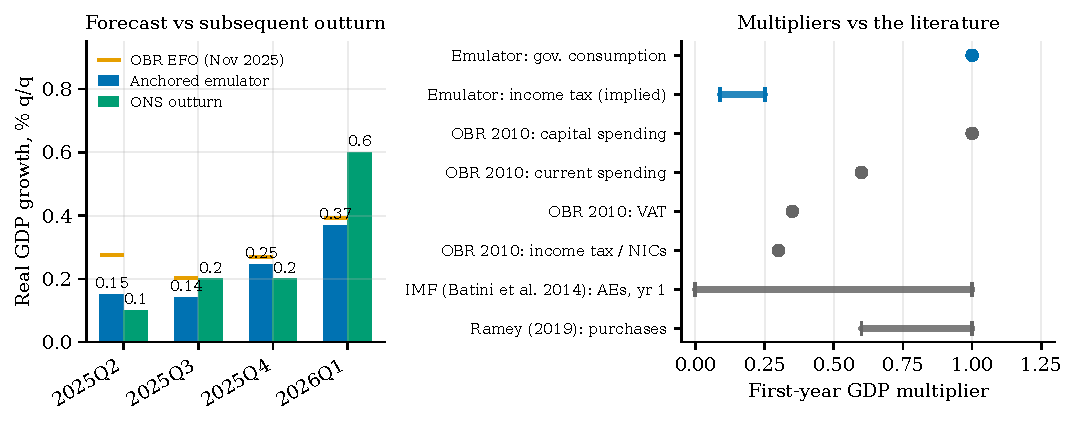
\includegraphics[width=\textwidth]{figures/fig_outturn.pdf}
\caption{Stepping outside the anchor vintage. Left: quarter-on-quarter real GDP growth, the November-2025-anchored emulator forecast (bars, with the published EFO path as markers) against ONS outturns published after anchoring \citep{ons2026gdp}. Right: the emulator's government-consumption multiplier and the implied income-tax multiplier of the 1p reform (impact to 2027Q4 range) against published first-year multiplier estimates: the interim OBR's June 2010 assumptions by instrument \citep{obr2010multipliers}, the IMF's bunching range for advanced economies in normal times \citep{batini2014}, and \citet{ramey2019}. Generated by \texttt{figures/fig\_outturn.py}; data in \texttt{figures/fig\_outturn\_data.csv}.}
\label{fig:outturn}
\end{figure}

\subsection{Multipliers against the published literature}
\label{sec:multlit}

Section~\ref{sec:experiments} reports the emulator's multiplier on government consumption as approximately 1.0 throughout---the mechanical demand-closure effect with both the import leakage (downward force) and the induced-income loop (upward force) inoperative. The right panel of Figure~\ref{fig:outturn} places that number, and the income-tax response, in the published range. The OBR's own multiplier assumptions, set out when the interim OBR costed the June 2010 consolidation and still its most explicit published statement, run from 0.3 for income-tax and NICs changes and 0.35 for VAT through 0.6 for current departmental and welfare spending to 1.0 for capital spending, tapering to zero over about five years as monetary policy and real wages adjust \citep{obr2010multipliers}. The IMF's guidance note recommends first-year multipliers of 0 to 1 for advanced economies in normal times, with spending measures toward the top of the range and revenue measures toward the bottom \citep{batini2014}, and \citet{ramey2019}, surveying the post-crisis empirical renaissance, puts the plausible range for aggregate government-purchases multipliers at 0.6 to 1.0. Against these, the emulator's $CGG$ multiplier of $\approx$1.0 sits at the top of the OBR's spending range---above the 0.6 the OBR would assume for a current-spending measure, for the reason Section~\ref{sec:experiments} documents: import leakage is switched off in this configuration, so the force that would pull the multiplier below one is absent. The income-tax side is more comfortable: the 1p reform's second-round GDP effect, expressed as a ratio to the $HHDI$ shock (both in per cent of GDP), implies a tax multiplier of 0.09 on impact rising to 0.25 by 2027Q4---approaching the OBR's 0.3 income-tax assumption from below as the consumption error-correction term cumulates, and inside the revenue end of the IMF range. The honest summary is that the emulator's multipliers are bracketed by, and mostly consistent with, the published assumptions, with the one out-of-range feature (no import leakage on the spending multiplier) both explained and flagged as future work.

\subsection{The policy costings record}
\label{sec:costingsdb}

A final check is against the official policy-costings record---the measure-by-measure database the OBR maintains alongside each EFO and the Treasury's certified costings documents. No recent fiscal event contains a basic-rate change to score against directly: the November 2025 Budget raised revenue through threshold freezes and rate changes on property, dividend, and savings income rather than the main rates \citep{hmt2025costings}, so HMRC's ready reckoner (Table~\ref{tab:comparison}, panel~B) remains the like-for-like benchmark for the worked reform. The nearest certified personal-tax measure is instructive on scale: the Budget's extension of the income-tax threshold freeze to 2030--31 is costed at \pounds 8.0 billion in 2029--30 \citep{hmt2025costings, obr2025efo}---the same order as the reckoner's \pounds 8.2 billion for 1p on the basic rate in 2028--29, and consistent with the well-known equivalence between freeze extensions and small rate rises under fiscal drag. The emulator's costing chain (PolicyEngine microdata to \pounds 6.5--7.4 billion for 1p) sits 10--15 per cent below both official numbers in the later years, for the microdata-versus-administrative-data reasons documented in Section~\ref{sec:results}; scoring the freeze extension itself through the bridge is a natural next validation exercise, since both the static costing and the OBR's certified number are published.
